\subsection{Results}
\label{sec:mpi:results}

These results show the attained speedups for the MPI implementation. Due to SeARCH limitations, only tests with two nodes were able to run (see \cref{sec:env, sec:method} for further details). Speedups are compared against the original sequencial version in \cref{fig:mpi:results}.

\begin{figure}[!htp]
	\centering
	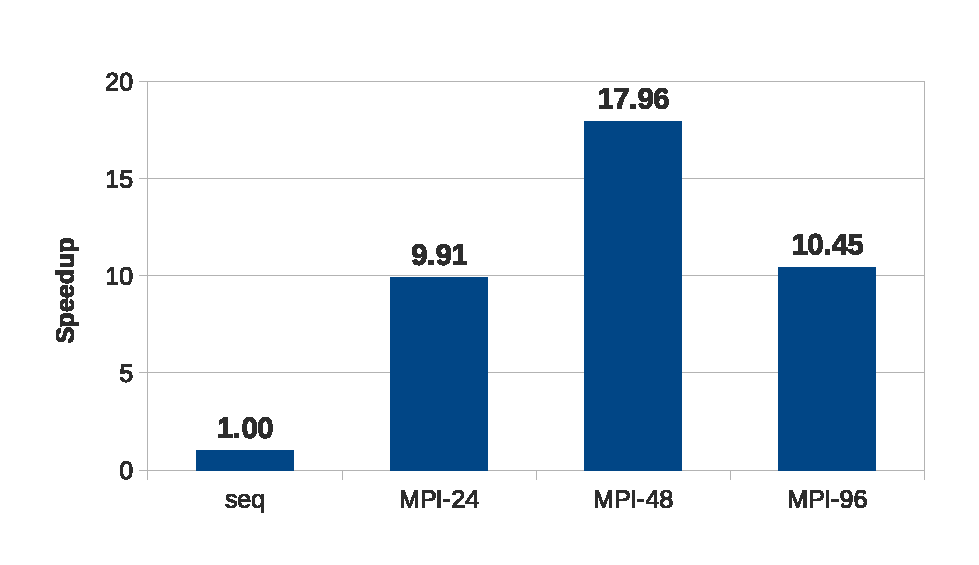
\includegraphics[width=\columnwidth]{graph_comparison_mpi}
	\caption{MPI implementation speedups}
	\label{fig:cuda:results}
\end{figure}

While there are actual speedups, especially for 48 processes, the results are not as good as the OpenMP results. The reason for this comes from the nature of the algorithm, that makes it very sensible to the overhead of communications. This imposes large limits to the scalability of any shared memory implementation of \polu.
